%杨舒云的实验报告编辑界面,使用了Huanyu Shi,2019级的模板,杨舒云在此拜谢ORZ!

%!TEX program = xelatex
\documentclass[dvipsnames, svgnames,a4paper,11pt]{article}
% ----------------------------------------------------- 
%	加边框的命令
%	参考:https://tex.stackexchange.com/questions/531559/how-to-add-the-page-border-for-first-two-pages-in-latex
\usepackage{tikz}
\usetikzlibrary{calc}
\usepackage{eso-pic}
\AddToShipoutPictureBG{%
\begin{tikzpicture}[overlay,remember picture]
\draw[line width=0.6pt] % 边框粗细
    ($ (current page.north west) + (0.6cm,-0.6cm) $)
    rectangle
    ($ (current page.south east) + (-0.6cm,0.6cm) $); % 边框位置
\end{tikzpicture}}


\usepackage{xcolor}
\definecolor{c1}{HTML}{475D7B} % 目录颜色 原版为2752C9 紫灰色535AAA 蓝紫色0B0DB7 深蓝色070F94 湖绿色219394 松石灰绿086173
\definecolor{c2}{HTML}{E26E1B} % 引用颜色(图片) 原版\definecolor{c2}{RGB}{190,20,83} 橙色F24729
\definecolor{c3}{HTML}{4DF8E8} % 新增颜色(表格)
\definecolor{c4}{HTML}{97C6C0} % 新增颜色(思考题)
\definecolor{c5}{HTML}{3E324A} % 新增颜色(推荐标记使用)

\usepackage{ctex}
\usepackage[top=28mm,bottom=28mm,left=15mm,right=15mm]{geometry}
\usepackage{hyperref} 
\hypersetup{
	colorlinks,
	linktoc = section, % 超链接位置,选项有section, page, all
	linkcolor = c1, % linkcolor 目录颜色
	citecolor = c1  % citecolor 引用颜色
}
\usepackage{amsmath,enumerate,multirow,float}
\usepackage{tabularx}
\usepackage{tabu}
\usepackage{subfig}
\usepackage{fancyhdr}
\usepackage{graphicx}
\usepackage{wrapfig}  
\usepackage{physics}
\usepackage{appendix}
\usepackage{amsfonts}

\usepackage{mathrsfs} % 字体

%
\usepackage{tcolorbox}
\tcbuselibrary{skins,breakable}
\newtcolorbox{tbox}[2][]{
    colframe=black!70!,
    breakable,
    enhanced,
	boxrule =0.5pt,
    title = {#2},
    fonttitle = \large\kaishu\bfseries,
	drop fuzzy shadow,
    #1
}
\newtcolorbox[auto counter,number within=section]{question}[1][]{
  top=2pt,bottom=2pt,arc=1mm,
  boxrule=0.5pt,
%   frame hidden,
  breakable,
  enhanced, %跨页后不会显示下边框
  coltitle=c1!80!gray,
  colframe=c3,
  colback=c4!3!white,
  drop fuzzy shadow,
  title={Reflection Question~\thetcbcounter:\quad},
  fonttitle=\bfseries,
  attach title to upper,
  #1
}

% ---------------------------------------------------------------------
%	利用cleveref改变引用格式,\cref是引用命令
\usepackage{cleveref}
\crefformat{figure}{#2{\textcolor{c2}{\textbf{Figure #1}}}#3} % 图片的引用格式
\crefformat{equation}{#2{(\textcolor{c2}{#1})}#3} % 公式的引用格式
\crefformat{table}{#2{\textcolor{c2}{\textbf{Table #1}}}#3} % 表格的引用格式


% ---------------------------------------------------------------------
%	页眉页脚设置
\fancypagestyle{plain}{\pagestyle{fancy}}
\pagestyle{fancy}
\lhead{\kaishu 中山大学 \quad 物理与天文学院 \quad 基础物理实验\uppercase\expandafter{\romannumeral2}} % 左边页眉
\rhead{Lab Report By 杨舒云 \& 戴鹏辉 } % 右边页眉
\cfoot{\thepage} % 页脚,中间添加页码


% ---------------------------------------------------------------------
%	对目录、章节标题的设置
\renewcommand{\contentsname}{\centerline{\Huge Outline}}
\usepackage{titlesec}
\usepackage{titletoc}
% \titleformat{章节}[形状]{格式}{标题序号}{序号与标题间距}{标题前命令}[标题后命令]
\titleformat{\section}{\centering\LARGE\songti}{}{1em}{}

% ---------------------------------------------------------------------
%   listing代码环境设置
\usepackage{listings}
\lstloadlanguages{python}
\lstdefinestyle{pythonstyle}{
backgroundcolor=\color{gray!5},
language=python,
frameround=tftt,
frame=shadowbox, 
keepspaces=true,
breaklines,
columns=spaceflexible,                   
basicstyle=\ttfamily\small, % 基本文本设置,字体为teletype,大小为scriptsize
keywordstyle=[1]\color{c1}\bfseries, 
keywordstyle=[2]\color{Red!70!black},   
stringstyle=\color{Purple},       
showstringspaces=false,
commentstyle=\ttfamily\scriptsize\color{green!40!black},%注释文本设置,字体为sf,大小为smaller
tabsize=2,
morekeywords={as},
morekeywords=[2]{np, plt, sp},
numbers=left, % 代码行数
numberstyle=\it\tiny\color{gray}, % 代码行数的数字字体设置
stepnumber=1,
rulesepcolor=\color{gray!30!white}
}




% ---------------------------------------------------------------------
%	其他设置
\def\degree{${}^{\circ}$} % 角度
\graphicspath{{./images/}} % 插入图片的相对路径
\allowdisplaybreaks[4]  %允许公式跨页 
\usepackage{lipsum}
\usepackage{adjustbox}
%\usepackage{mathrsfs} % 字体
\captionsetup[figure]{name=Figure} % 图片形式
\captionsetup[table]{name=Table} % 表格形式

\usepackage{enumitem}
\usepackage{tabularray}  %绘制表格时可以更加方便添加框线
\usepackage{xcolor} %添加更多文本颜色


%---------------------------------------------------------------------
%	正文
%---------------------------------------------------------------------



\begin{document}
	
	
	
	% 实验报告封面	
	
	% 顶栏
	
	% ---
	
	% 信息栏
	\begin{table}
		\renewcommand\arraystretch{1.7}
		\centering
		\begin{tabularx}{\textwidth}{|X|X|X|X|}
			\hline
			专业: & 物理学 & 年级: & 2022级 \\
			\hline
			姓名: & 戴鹏辉、杨舒云 & 学号: & 22344016、22344020\\
			\hline
			室温: & 26\degree C & 实验地点: & A515 \\
			\hline
			学生签名:& 见\textbf{附件} & 评分: &\\
			\hline
			实验时间:& 2024/6 & 教师签名:&\\
			\hline
		\end{tabularx}
	\end{table}
	% ---
	
	% 大标题
	\begin{center}
		\LARGE Lab2-S.A.M. \quad 设计性实验“热力学第二定律”实验计划与方案\\Heat Engine Design Based on Thermoelectric Effect and Verification Experiment of The Second Law of Thermodynamics
	\end{center}
	
	\textbf{【回顾实验要求(Review)】}
	\begin{enumerate}
		\item 目的
		
		设计并实现输出功率在1瓦以上的“热机”,以探究和验证热力学第二定律。
		
		\item 要求
		\begin{enumerate}
			\item \textbf{学习和理解热电效应}:
			\begin{itemize}
				\item 包括Seebeck效应、Peltier效应和Thomson效应。
				\item 设计实验方案,包含原理和物理模型。
			\end{itemize}
			
			\item \textbf{制作热机}:
			\begin{itemize}
				\item 展示热力学第二定律的“热机”。
				\item 电或机械输出功率不低于1瓦。
			\end{itemize}
			
			\item \textbf{测量与分析}:
			\begin{itemize}
				\item 测量装置的最大输出功率和输出效率。
				\item 讨论实际结果与Carnot循环的差异。
				\item 探讨进一步提高效率的方法。
				\item 分析测量精度和不确定度。
			\end{itemize}
			
			\item \textbf{确保安全性}:
			
			确保装置表面(可触摸到的部分)温度不高于50\degree C。
			
		\end{enumerate}
	\end{enumerate}
	% ---
	
	% 注意事项
	
	% 基本
	%\textbf{【实验报告注意事项(Precautions)】}
	
	
	% 安全
	%\textbf{【实验安全注意事项(Safety)】}	
	
	
	% ---
	
	% 特别鸣谢
	\textbf{【特别鸣谢及模板说明(Special Thanks)】}	
	
	感谢2019级学长石寰宇为本实验报告提供\LaTeX 模板。\textcolor{red}{\textbf{由于原实验报告模板缺少实验编号,为方便在电脑上整理,故添加自命名编号Lab2-S.A.M.。}}除此以外,本实验报告正在向全文用英文表达的方向改进,在此期间可能会出现中英夹杂的情况,望老师海涵!
	% ---
	
	
	
	% 目录
	\clearpage
	\tableofcontents
	\clearpage
	% ---
	
	
	
	% 预习报告	
	
	% 小标题
	\setcounter{section}{0}
	\section{Lab2-S.A.M. 基于热电效应的热机设计与热力学第二定律验证实验\\ \quad\heiti 实验原理(Principle)}
	% ---
	
	% 实验目的
	\subsection{实验目的(Purpose)}
	\begin{itemize}
		\item \textbf{开路输出电压与温差的关系}:
		
		Seebeck效应,器件的等效热电系数 $\alpha$ 和等效热导 $\lambda$(热阻 $\rho$)。
		
		\item \textbf{特定负载下输出功率与温差的关系}:
		
		验证热力学第二定律。
		
		\item \textbf{热源功率和单片热电堆输出效率的优化}:
		
		在给定热源功率下,优化室温条件下单片热电堆的输出效率。
		
		\item \textbf{固定冷、热源温度下的测量}:
		\begin{itemize}
			\item 测量在不同负载下的热电机输出功率与输出效率的关系。
			\item 分析器件内阻 $r$。
		\end{itemize}
	\end{itemize}
	% ---
	
	% 原理概述
	\subsection{原理概述(Principle)}
	\begin{enumerate}
		\item Seebeck效应
		
		当两种不同的导体或半导体连接成回路,并且两个接头的温度不同,就会在回路中产生电动势。
		
		\begin{figure}[htbp]
			\centering
			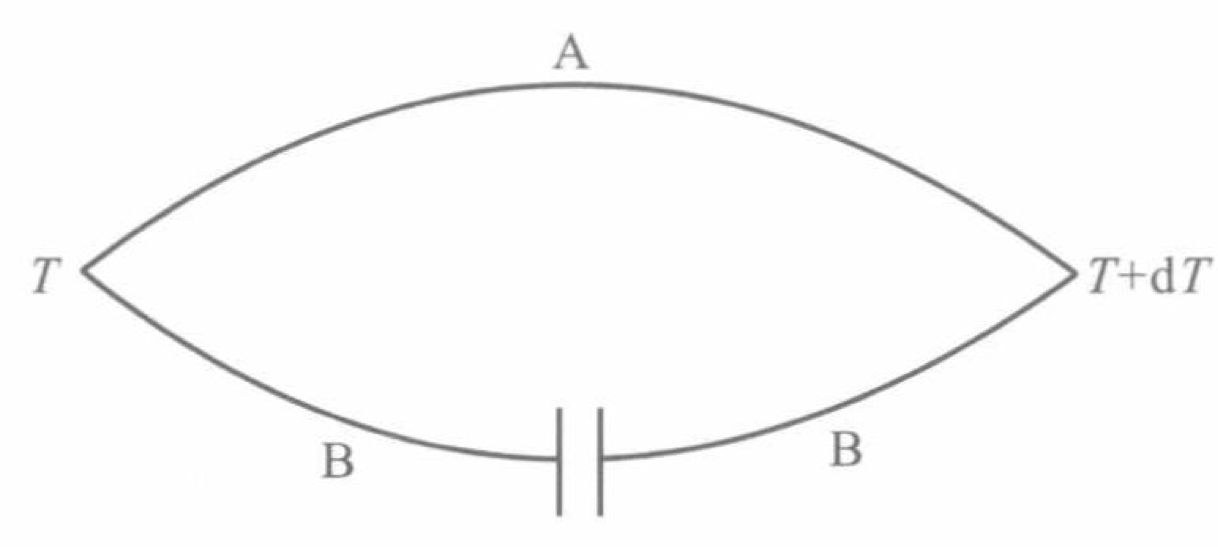
\includegraphics[width=0.45\textwidth]{SamPre_1_Gra1.jpg}
		\end{figure}
		
		$$\mathrm{d}V=\epsilon_{AB}\mathrm{d}T$$
			
		其中,$\epsilon_{AB}$是温差电动势系数(又称Seebeck系数,记为$\alpha$)。符号约定为如果在高温段电动势驱使电流由金属A流向金属B为正。	
		
		\item Peltier效应
		
		当电流通过两种不同材料组成的电路时,一个接头会吸热,另一个接头会放热。这个效应对于调控热机的温度非常重要,尤其是在确保装置表面温度不超过50\degree C的安全要求下。
		
		\begin{figure}[htbp]
			\centering
			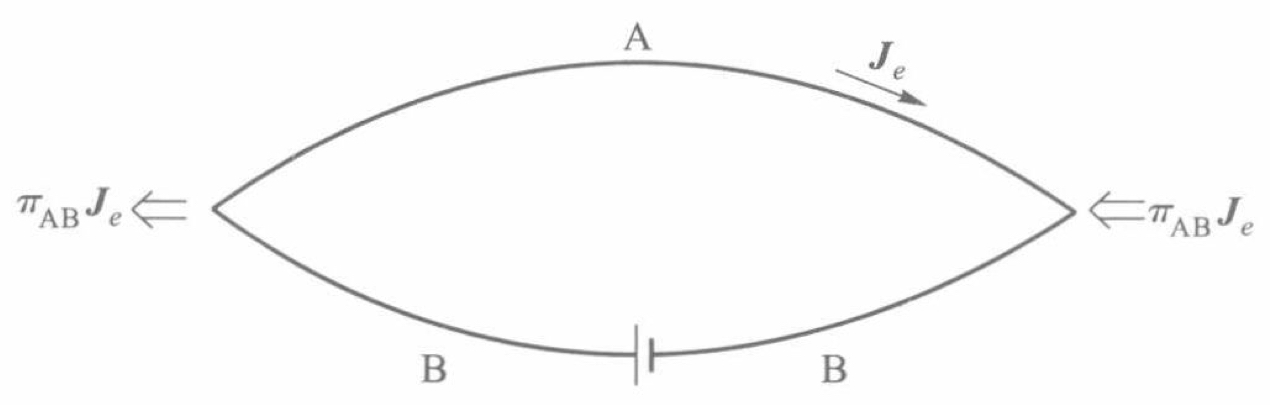
\includegraphics[width=0.5\textwidth]{SamPre_1_Gra2.jpg}
		\end{figure}
		
		$$\textbf{J}_{q\pi}=\pi_{AB}\textbf{J}_{e}$$
		
		其中,$\textbf{J}_{q\pi}$是Peltier热流密度,$\textbf{J}_{e}$是从A到B的电流密度,$\pi_{AB}$是两种金属的Peltier系数(与温度有关)。
		
		\item Thomson效应
		
		在均质导体中,如果存在温度梯度,当电流通过时,会伴随着吸热或放热的现象。这对于完整的热电模型和效率分析很关键。$\dot{Q}=\mu I\cdot \nabla T$,$\mu$为Thomson系数。
		
		\item 热电模型参数
		
		\begin{itemize}
			\item 等效热导表示材料传导热量的能力,单位通常为瓦每米每开尔文(W/m·K)。等效热导越大,材料的热传导能力越强。
			$
			\lambda = \frac{Q}{A \cdot \Delta T \cdot t}
			$。
			其中,$\lambda$ 是等效热导(W/m·K),$Q$ 是通过材料的热量(J),$A$ 是材料的横截面积($m^2$),$\Delta T$ 是材料两端的温差(K),$t$ 是热量传导所需的时间(s)。
			通过Fourier热传导定律,也可以表示为(其中 $L$ 是材料的长度(m)):
			$
			Q = \lambda \cdot A \cdot \frac{\Delta T}{L} \cdot t
			$。
			
			\item 热阻表示材料对热流阻碍的能力,单位通常为开尔文每瓦(K/W)。热阻越大,材料的热流阻碍能力越强。
			$
			R_{\text{th}} = \frac{\Delta T}{Q}
			$。
			其中,$R_{\text{th}}$ 是热阻(K/W),$\Delta T$ 是材料两端的温差(K),$Q$ 是通过材料的热量(W)。
			
			\item 等效热导和热阻是互为倒数的关系:
			$
			R_{\text{th}} = \frac{L}{\lambda \cdot A}
			$,
			$
			\lambda = \frac{L}{R_{\text{th}} \cdot A}
			$。
		\end{itemize}
		
		\item Seebeck效应电源的外输出特性
		
		\begin{itemize}
			\item 开路电压是指没有外部负载连接时,热电发电装置两端的电压。根据Seebeck效应,开路电压与温差成正比,$V_{\text{oc}} = \alpha \Delta T$。
			
			\item 当热电发电装置连接到负载时,输出电压会由于内阻的存在而下降。负载电压$V_{\text{L}} = \frac{\alpha \Delta T \cdot R_{\text{L}}}{R_{\text{L}} + R_{\text{in}}}$,而输出功率是负载上消耗的功率$P_{\text{out}} = \frac{(\alpha \Delta T)^2 \cdot R_{\text{L}}}{(R_{\text{L}} + R_{\text{in}})^2}$。
			
			\item 当负载电阻等于内阻时,热电发电装置输出的功率达到最大$P_{\text{max}} = \frac{(\alpha \Delta T)^2}{4 R_{\text{in}}}$。				
		\end{itemize}
		
		\item 电加热器
		
		电加热器(电热贴)通过电能转化为热能来实现加热,其工作原理基于焦耳定律$Q = I^2 R t$。
		
		使用电压表并联连接在电加热器两端,读取电压值;使用电流表串联连接在电路中,读取电流值;根据测得的电压和电流,使用公式$P = VI$计算加热功率。
		
		或者采用使用欧姆表测量电加热器的电阻,使用测得的电阻和电流计算$P = I^2 R$。
		
		对于电流电压随时间变化的情况,计算一段时间的总热功可以利用积分来实现。
		
		\clearpage
		\item PID控温
		
		\begin{table}[htbp]
			\centering
			\begin{tabular}{|c|c|c|}
				\hline
				控温算法 & 优点 & 缺点 \\
				\hline
				PID 控制 & 简单、易实现 & 性能有限,难以处理复杂系统 \\
				\hline
				模糊控制 & 不需要精确模型,适应性强 & 规则设计复杂,性能依赖于规则质量 \\
				\hline
				模型预测控制 & 最优性能,多变量处理 & 计算量大,依赖系统模型 \\
				\hline
				自适应控制 & 参数自调整,适应性强 & 实现复杂,收敛性问题 \\
				\hline
				神经网络控制 & 非线性处理能力强 & 训练复杂,数据需求大 \\
				\hline
				最优控制 & 理论性能优 & 实现复杂,计算量大 \\
				\hline
			\end{tabular}				
		\end{table}
		
		先考虑采用最经典的PID控温
		
		\begin{itemize}
			\item PID(Proportional-Integral-Derivative)控制是一种用于温度控制的经典算法,通过对误差的比例、积分和微分进行计算和调整,精确控制加热器的输出,从而实现温度的稳定控制。PID 控制器通常由三个部分组成:比例(P),积分(I),和微分(D)。
			
			\item PID 控温的控制量 $u(t)$ 可以表示为:$$u(t) = K_p e(t) + K_i \int_0^t e(\tau) d\tau + K_d \frac{d e(t)}{dt}$$
			
			\item 比例控制$P_{\text{out}} = K_p e(t)$直接与当前误差成比例,调整系统响应速度;积分控制$I_{\text{out}} = K_i \int_0^t e(\tau) d\tau$对误差进行积分,消除稳态误差,增强系统的长期精度;微分控制$D_{\text{out}} = K_d \frac{d e(t)}{dt}$对误差进行微分,预测误差变化趋势,减小超调和振荡。
		\end{itemize}
		
		在实际应用中,PID 控制通常以离散形式实现。离散 PID 控制算法如下:			
		\[
		u[k] = u[k-1] + K_p (e[k] - e[k-1]) + K_i e[k] + K_d \left( \frac{e[k] - e[k-1]}{T} \right)
		\]
		其中:
		\begin{itemize}
			\item $u[k]$ 是第 $k$ 次采样时的控制输出;
			\item $e[k]$ 是第 $k$ 次采样时的误差;
			\item $T$ 是采样周期。
		\end{itemize}
		
		\item 测量(估算)热对空气的耗散
		
		\begin{enumerate}
			\item 热对流:使用牛顿冷却定律($\dot{Q}=hA(T_{surface}-T_{air})$),A为面积。
			\item 热辐射:使用斯特藩-玻尔兹曼定律($\dot{Q}=\epsilon\sigma A(T^4_{surface}-T^4_{air})$),A为面积。				
		\end{enumerate}
	\end{enumerate}
	% ---
	
	% 实验方案
	\subsection{实验方案(Scheme)}
	\subsubsection{整体规划}
	\begin{enumerate}
		\item 各元件性能测量
		\begin{itemize}
			\item Seebeck效应测量:通过改变温差并测量开路电压来研究Seebeck效应,从而确定$\alpha$;
			\item 器件内阻的测量与影响:内阻对热电转换效率有重要影响,了解并优化内阻对提高热机性能是必要的;
			\item 考虑测量电加热器的加热功率(以及其它元件性能,如Peltier效应)。
		\end{itemize}
		
		\item 搭建热机
		\begin{itemize}
			\item 热电堆集成——电加热器与Seebeck元件,测控部分——PID控温(热端、冷端),输出电路部分(输出功率测量)。
		\end{itemize}
		
		\item 负载与效率测量
		\begin{itemize}
			\item 加热功率测控——电流表电压表实时测控(含于PID系统中,编写相关程序);
			\item 输出功率测控——电流表电压表实时测控(考虑是否编程);
			\item 测量最大输出功率——改变输出电路的负载;
			\item 测量最大输出效率——改变温差与负载,优化其它部分;
			\item 探究如何测量热端的损失。
		\end{itemize}
		
		\item 热力学第二定律的展示
		\begin{itemize}
			\item 通过实验测量,展示即使是优化过的热电装置,其效率也受到卡诺效率的限制,这直接体现了热力学第二定律。
			\item 讨论如何通过实验设计来逼近卡诺效率,包括使用最佳材料、最佳温差和最佳负载条件。
		\end{itemize}			
		
		\item 结论与进一步的探索
		\begin{itemize}
			\item 比较热机效率与理论卡诺效率的差异,讨论可能的优化途径和技术挑战;
			\item 探究各部分如何优化(热电堆——减小散热,增大温差,冷热端优化;测控——优化控温算法,改进实时测量程序;输出电路部分——减小散热,考虑Thomson效应的影响;理论建模——估算散热进一步修正)。
		\end{itemize}
	\end{enumerate}
	
	\begin{figure}[htbp]
		\centering
		\subfloat[]{
			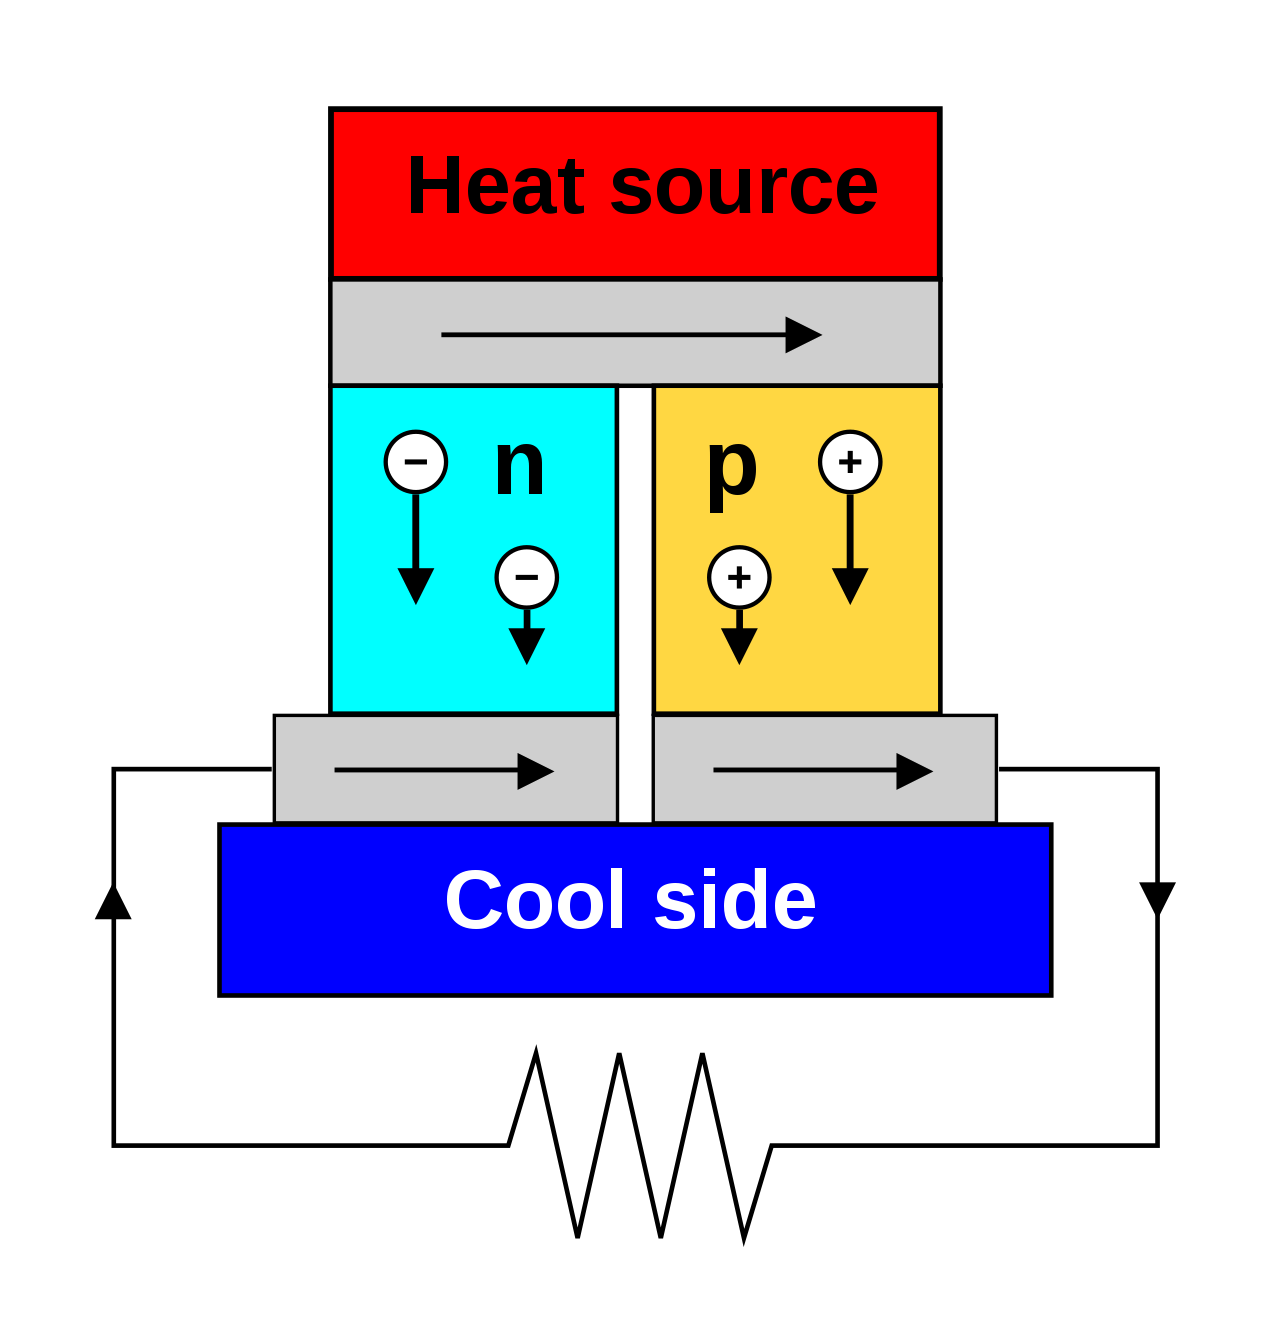
\includegraphics[width=0.4\textwidth]{SamPre_1_Gra3.png}
		}
		\subfloat[]{
			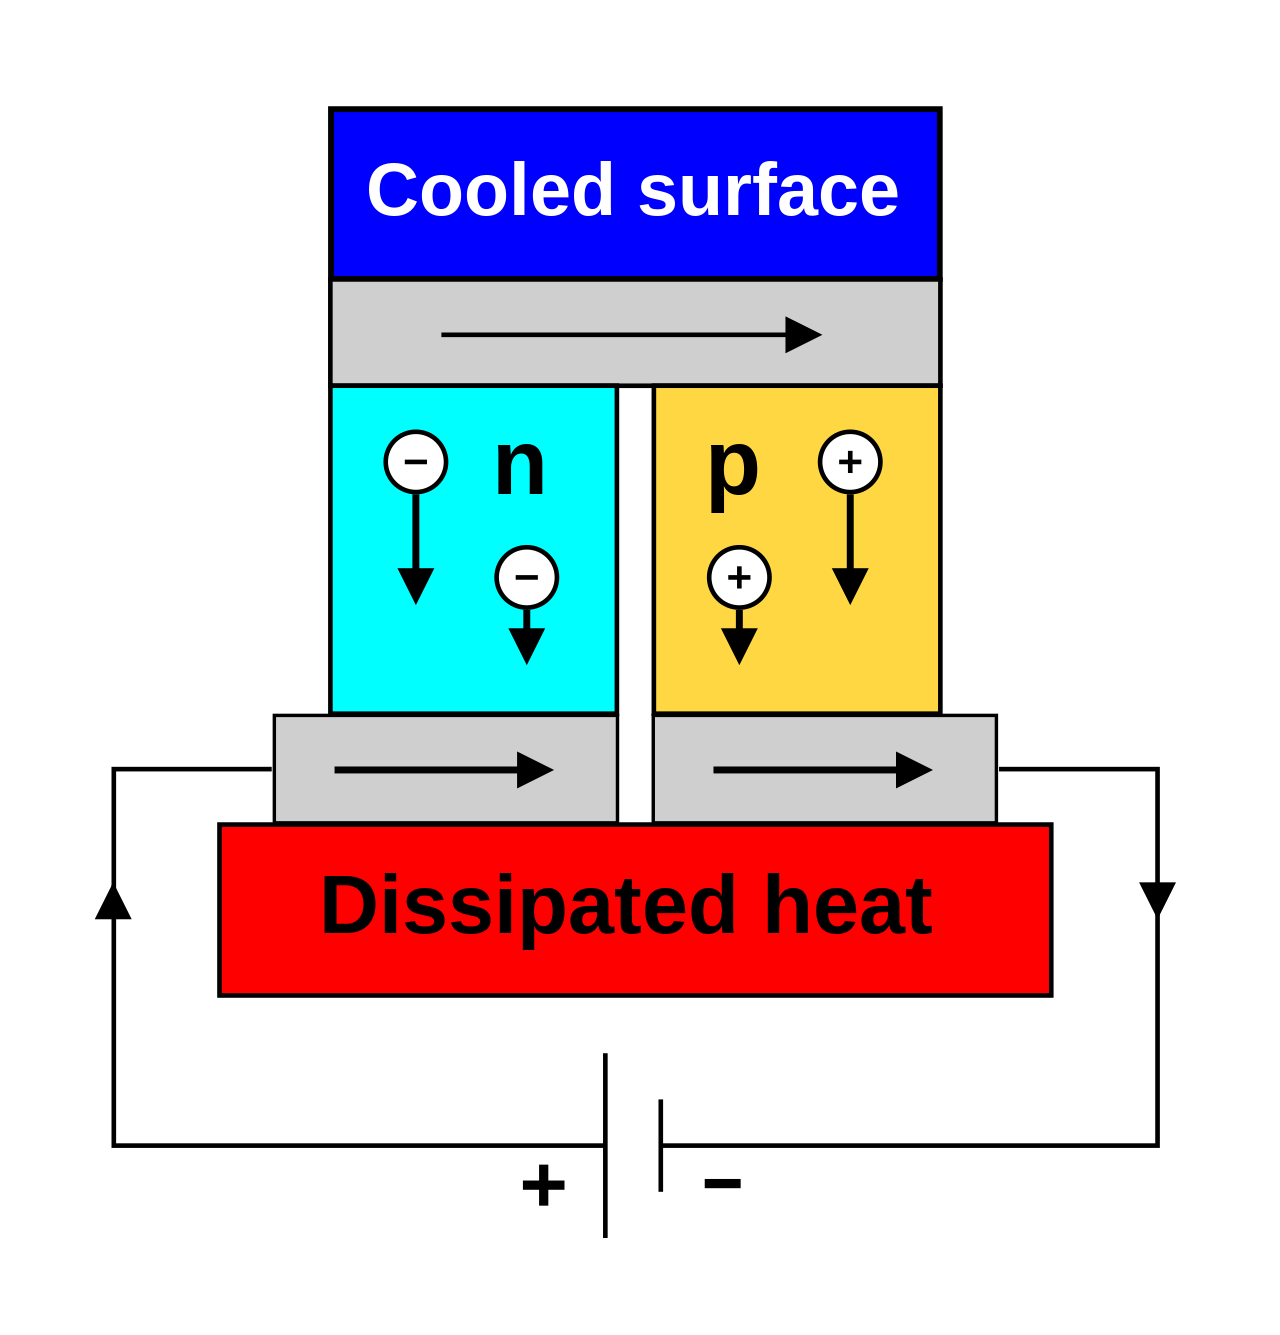
\includegraphics[width=0.4\textwidth]{SamPre_1_Gra4.png}
		}	
	\end{figure}
	
	\subsubsection{热机搭建}
	
	\begin{enumerate}
		\item 热电模块配置:将若干热电模块串联,以增加输出电压。根据需要的输出功率和单个热电模块的性能,计算所需模块的数量。并联可以增加输出电流。
		
		\item 热源与冷却系统安装:
		\begin{itemize}
			\item 将电加热器固定在热电模块的一侧作为热源,保证热端能够获得足够高的温度。
			\item 在热电模块的另一侧安装冷却系统,保持冷端的温度尽可能低。
		\end{itemize}				
		
		\item 电气连接与测量:
		\begin{itemize}
			\item 将电压表和电流表并联/串联到热电模块或模块组合的输出端,以便测量输出电压和电流。
			\item 将负载连接到热电模块的输出端,开始时可以使用一个较高的电阻值作为基准。
		\end{itemize}
		
		\item 温度监控与安全保障:
		\begin{itemize}
			\item 在热端和冷端分别安装温度传感器,实时监控温度,确保热端温度在安全范围内,且冷端不会过热。
			\item 使用绝缘材料和防护措施确保操作者不会直接接触到高温部分。
		\end{itemize}
		
		\item 输出功率的测量与优化:
		\begin{itemize}
			\item 逐步调整负载电阻,测量不同负载条件下的输出功率,找到输出功率最大时的负载电阻值。
			\item 记录最优负载条件下的输出电压、电流和功率,验证是否达到或超过1W的输出。
		\end{itemize}
	\end{enumerate}
	
	\subsubsection{温度控制}
	
	控制冷端与热端温度恒定 ,一方面可用于计算卡诺机效率,另一方面便于计算吸收热量。
	
	\begin{enumerate}
		\item 温度监测
		
		在热端和冷端分别安装高精度的温度传感器,如热电偶或PT100传感器,以实时监测温度。
		
		\item 热端温度控制
		\begin{itemize}
			\item 可控加热源:使用可调节的加热设备(如电加热器)来精确控制热端温度。结合PID控制器可以根据温度传感器的反馈自动调整加热功率,以保持目标温度。
			\item 隔热材料:在热端周围使用高效的隔热材料减少热损失,有助于维持稳定的温度。
		\end{itemize}
		
		\item 冷端温度控制
		\begin{itemize}
			\item 主动冷却系统:将另一个温度传感器安装在冷端,将其输出连接到控制冷端温度的PID控制器。对于Peltier制冷方案,PID控制器的输出控制Peltier元件的工作电流。对于水冷方案,PID控制器调节水泵的流速或风扇的转速,根据冷端温度与目标温度的偏差来调整冷却强度,维持冷端温度。
			
			\item 热管理策略:优化散热器的设计(如增加散热片、使用热管技术),以提高冷端的散热效率。
		\end{itemize}
		
	\end{enumerate}
	
	\subsubsection{测量热机效率}
	
	\begin{enumerate}
		\item 测量输出电功率
		
		使用电流表和电压表测量热电模块(和电加热器)的输出电流(I)和电压(V)。 
		
		\item 测量输入热功率
		\begin{itemize}
			\item 直接法:如果使用热流计,直接测量输入到热机的热流量(Q)。然后,根据加热源工作的时间(t),计算输入的热功率。
			\item 间接法:如果没有热流计,可以通过测量加热源的电功率和效率来估算输入的热功率。
		\end{itemize}
		
		\item 测量温度差
		
		使用温度传感器测量热端和冷端的温度,以评估热机工作的温度差。
		
		\item 计算效率
		
		使用测得的电功率和热功率计算热机的效率。
		
	\end{enumerate}
	
	% 仪器用具
	\clearpage
	\subsection{仪器用具(Instruments)}
		\begin{table}[htbp]
			\centering
			\renewcommand\arraystretch{1.6}
			% \setlength{\tabcolsep}{10mm}
			\begin{tabular}{p{0.05\textwidth}|p{0.20\textwidth}|p{0.05\textwidth}|p{0.5\textwidth}}
				\hline
				编号& 仪器用具名称 & 数量 &  主要参数(型号,测量范围,测量精度等) \\
				\hline
				1& TEC片 & >1 & Seebeck-TEC1-12703 \\
				2& 风扇 & 1 & -- \\
				3& 加热电阻 & 1 & -- \\
				4& 导热硅脂 & 大量 & -- \\
				5& 直流稳压电源 & 1 &  \\
				6& my-DAQ元件 & >1 & -- \\
				7& 导线 & 大量 & -- \\
				8& 铜片 & >2 & -- \\
				9& 绝热材料 & 大量 & -- \\
				10& 软件控制平台 & >1 & -- \\
				11& PT100测温电阻 & >1 & -- \\
				12& 其它 & 待定 & -- \\
				\hline
			\end{tabular}
		\end{table}
	
	\quad
	
	\begin{figure}[htbp]
		\centering
		\subfloat[]{
			
\includegraphics[width=0.2\textwidth]{SamPre_1_Gra5.jpg}
		}
		\subfloat[]{
			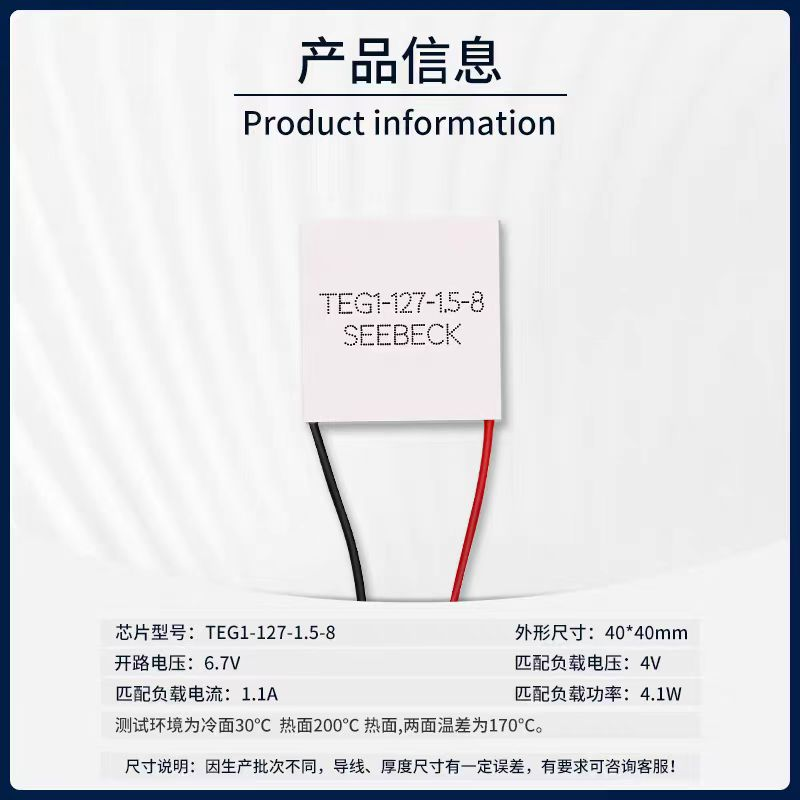
\includegraphics[width=0.2\textwidth]{SamPre_1_Gra6.jpg}
		}	
	\end{figure}
	
	% ---
	
	% 实验前思考题
	%\subsection{实验前思考题(Questions)}
	
	% ---
	
	
	
	% 实验记录(实验进度)
	\clearpage
	
	% 顶栏
	
	% ---
	
	% 小标题
	\section{Lab2-S.A.M. 基于热电效应的热机设计与热力学第二定律验证实验\\ \quad\heiti 实验进度(Progress)}
	% ---
	
	目前已经初步搭建好热机的主体部分,并编写好温度测量程序,然后进行了热机首次工作测试并测量了负载曲线,结果如下所示。
	
	\begin{figure}[htbp]
		\centering
		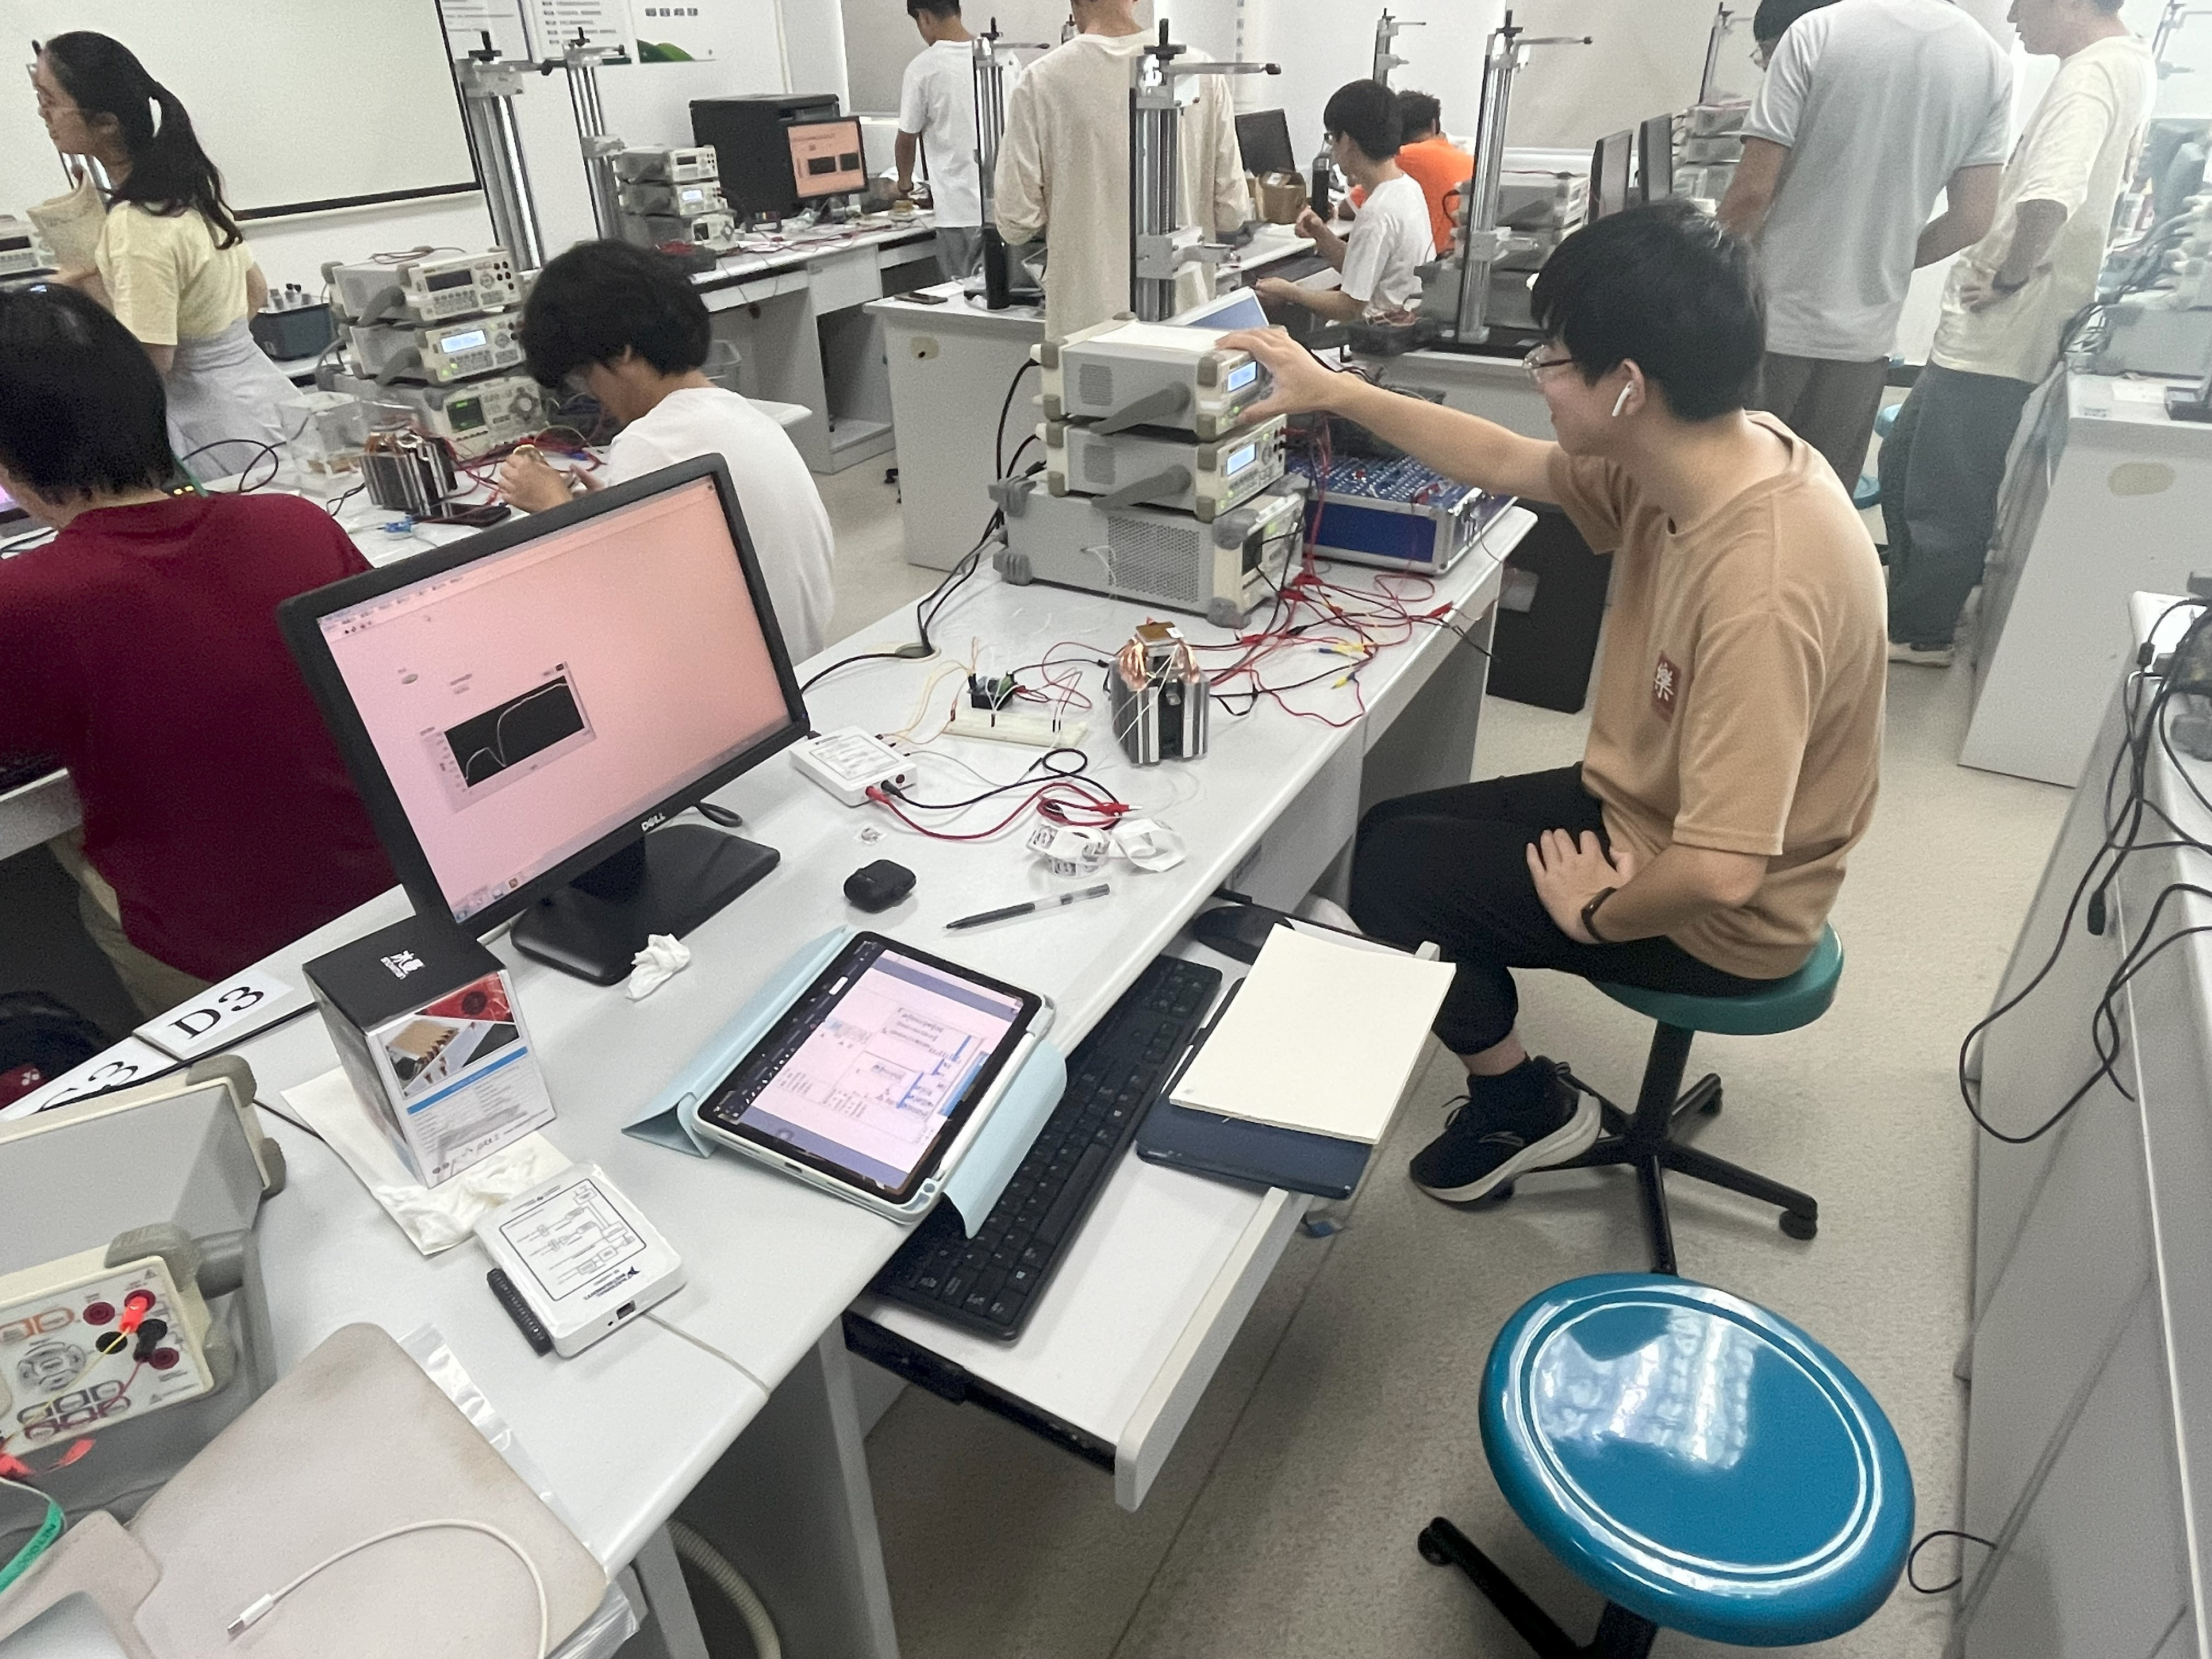
\includegraphics[width=0.65\textwidth]{S.A.M._Report1_Gra1.jpg}
	\end{figure}
	
	\begin{figure}[htbp]
		\centering
		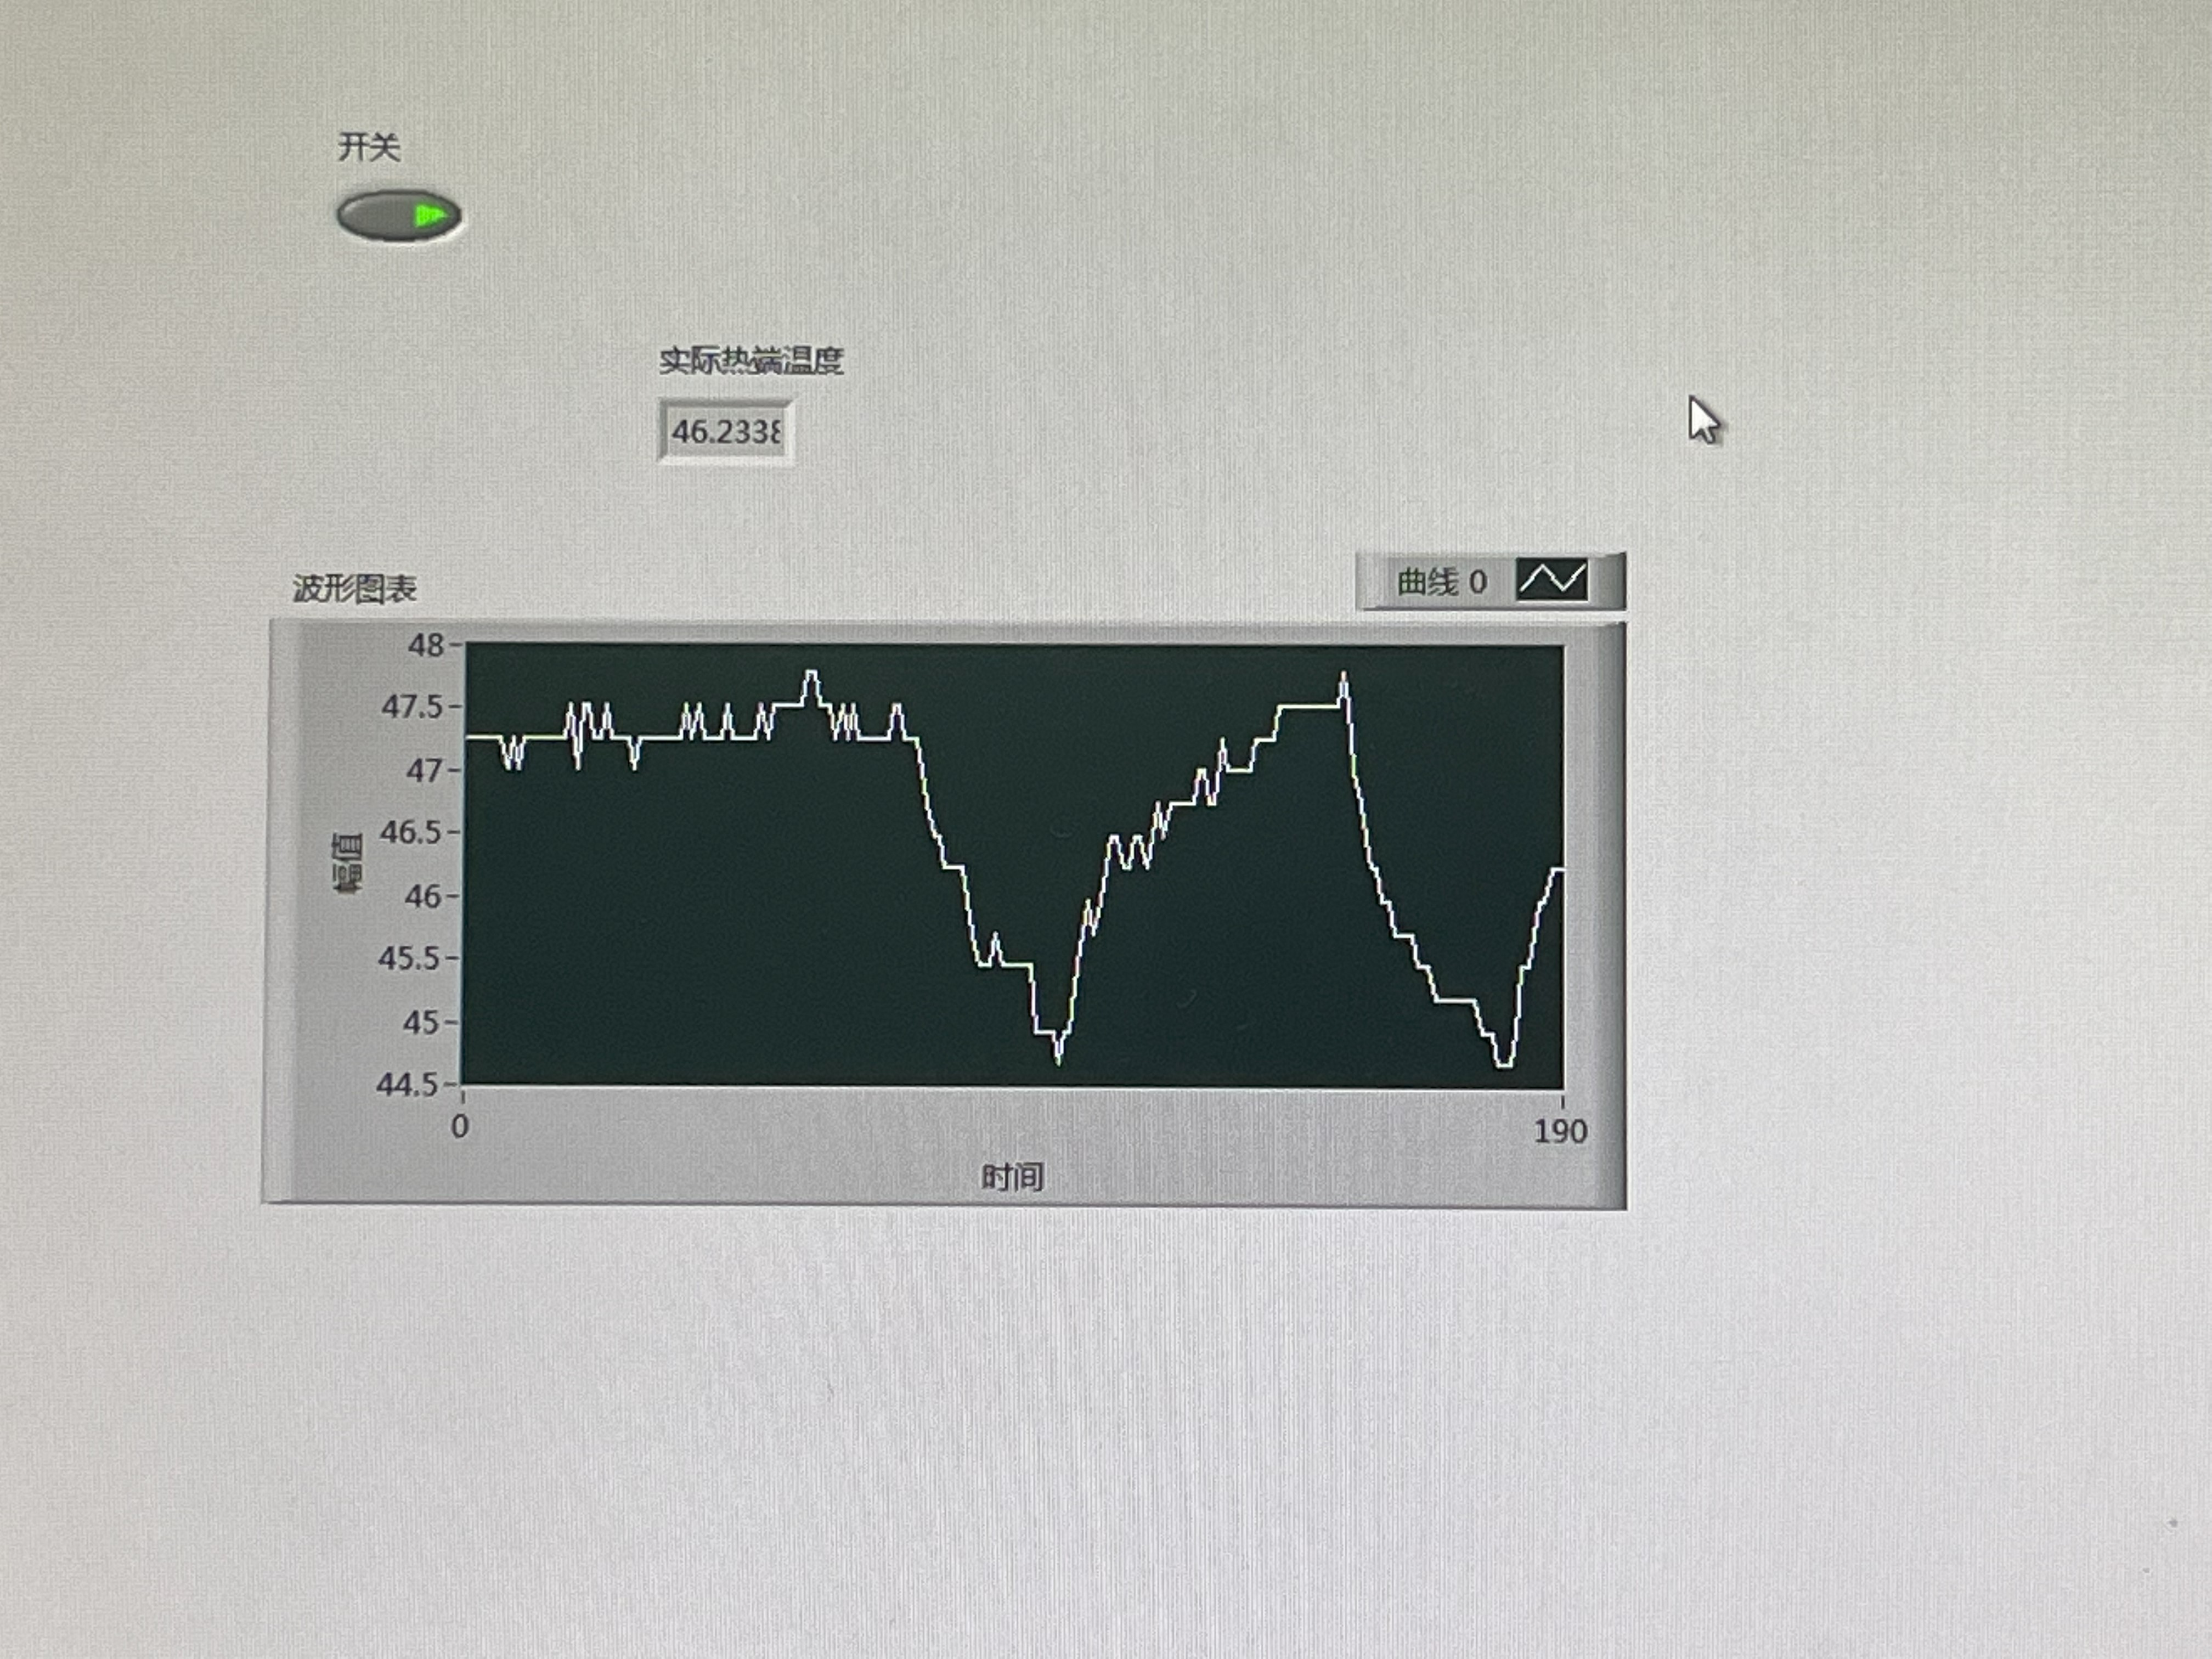
\includegraphics[width=0.65\textwidth]{S.A.M._Report1_Gra2.jpg}
	\end{figure}
	
	\clearpage
	\begin{figure}[htbp]
		\centering
		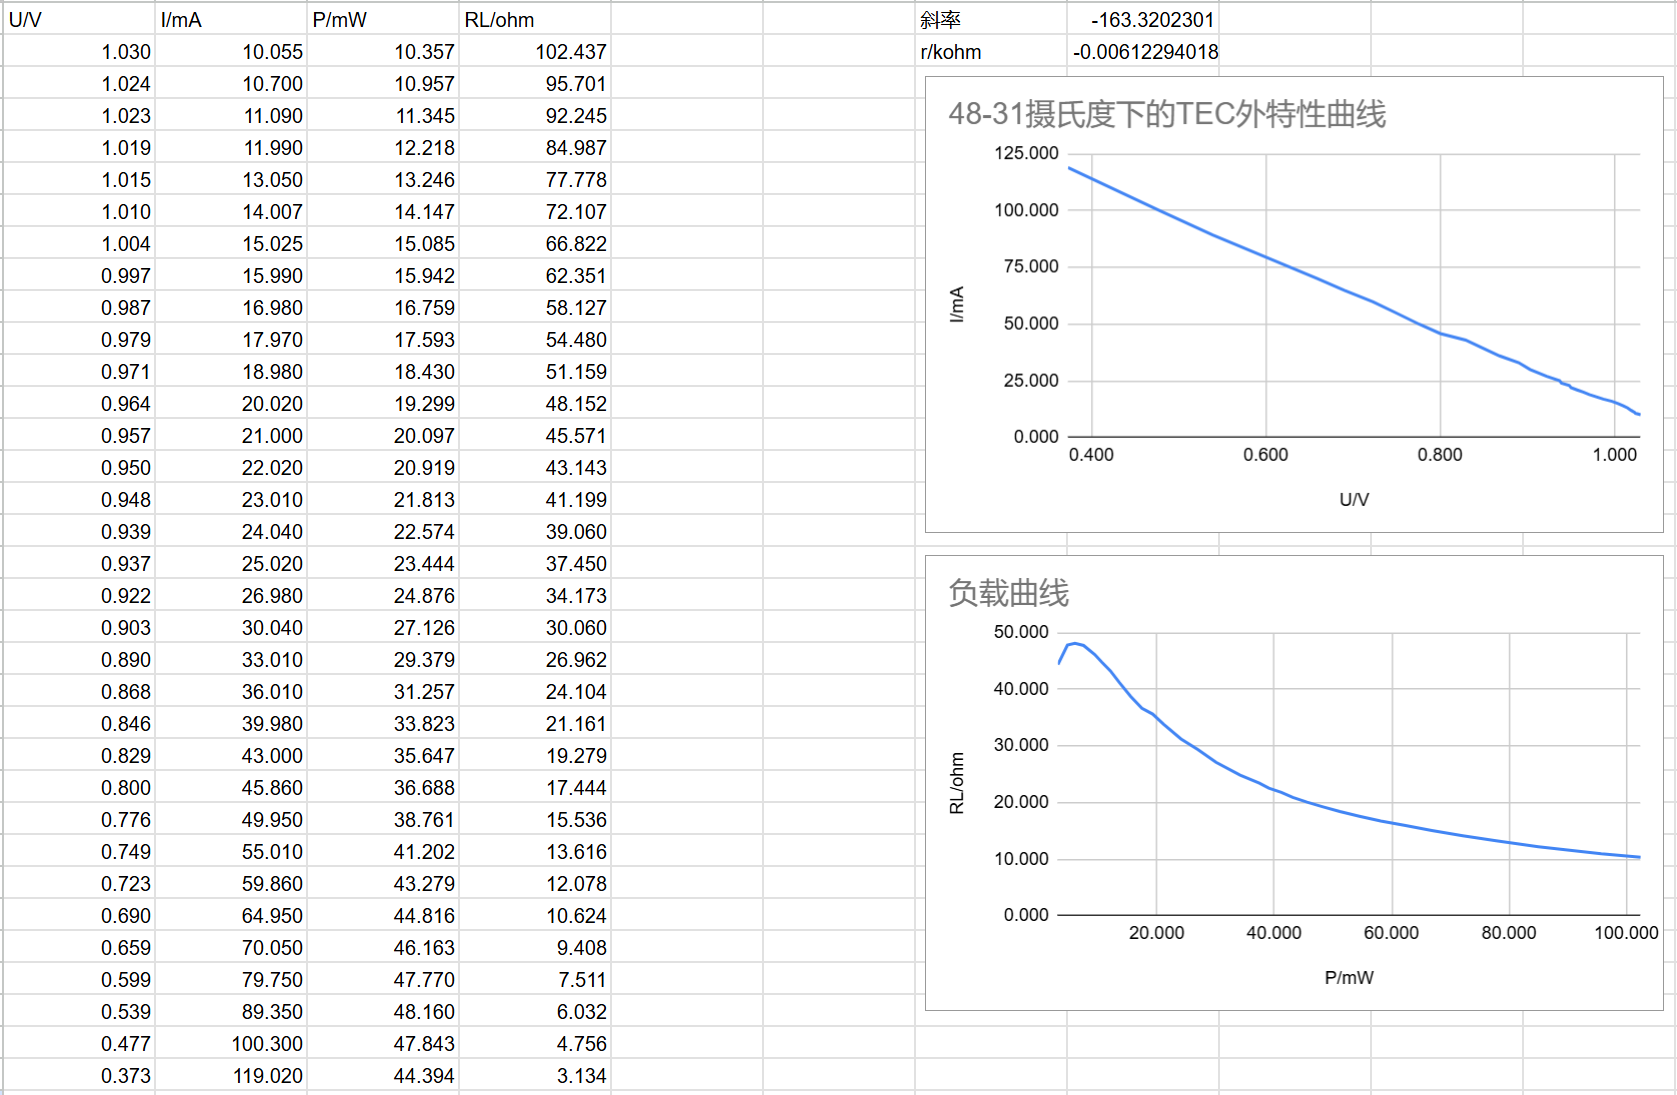
\includegraphics[width=\textwidth]{S.A.M._Report1_Gra3.png}
	\end{figure}
	
	% 实验过程记录
	%\subsection{实验内容、步骤与结果(Content, Procedures \& Results)}
	
	%
	%\subsubsection{操作步骤记录(Operations)}
	
	%
	%\subsubsection{实验结果展示(Display)}
	
	% ---
	
	% 原始数据
	%\clearpage
	%\subsection{原始数据记录(Original Data)}
	%The original data in the experimental notebook is shown in %\cref{} (signed).
	
	%See the \textbf{Attachment} section for the arrangement of the experimental bench desktop (%\cref{}).
	
	%Other raw data are shown in %\cref{}.
	% ---
	
	% 问题记录
	%\subsection{实验过程中遇到的问题记录(Difficulties)}
	
	% ---
	
	
	
	% 分析与讨论(后续规划)
	%\clearpage
	
	% 顶栏
	
	% ---
	
	% 小标题
	\section{Lab2-S.A.M. 基于热电效应的热机设计与热力学第二定律验证实验\\ \quad\heiti 后续规划(Expectation)}
	% ---
	
	后续规划如下:
	\begin{enumerate}
		\item 完善热机:
		\begin{enumerate}
			\item 增大冷端热端温差;
			\item 为热端加装绝热装置;
			\item 考虑对TEC片的集成,提高对加热电阻的利用率;
		\end{enumerate}
		
		\item 关于负载曲线的研究:
		\begin{enumerate}
			\item 我们在进行初次负载曲线测量时发现了在外负载接近短路时出现了一些反常现象,可以进一步对此研究;
			\item 测量在不同温度下的外负载曲线;
		\end{enumerate}
		
		\item 验证热力学第二定律
		\begin{enumerate}
			\item 测量不同温度下的负载曲线;
			\item 测量不同温度下的热机效率;
			\item 考虑进一步提高热机效率。
		\end{enumerate}
		
	\end{enumerate}
	
	% 数据处理
	%\subsection{实验数据分析(Analysis)}
	
	% ---
	
	% 实验后思考题
	%\subsection{实验后思考题(Questions)}
	
	% ---
	
	
	% 结语部分
	%\clearpage
	
	% 小标题
	\section{Lab2-S.A.M. 基于热电效应的热机设计与热力学第二定律验证实验\\ \quad\heiti 结语(The End)}
	% ---
	
	% 总结、杂谈与致谢
	%\subsection{总结、杂谈与致谢(Summary, Thoughts \& Thanks)}
	
	% ---
	
	% 参考文献
	\subsection{参考文献(References)}
	[1] 维基百科 https://zh.wikipedia.org
	
	[2] 沈韩.基础物理实验.——北京:科学出版社,2015.2 ISBN:978-7-03-043311-4
	
	% ---
	
	% 附件
	\subsection{附件(Attachment)}
	%The arrangement of the experimental bench desktop is shown in %\cref{}.
	
	%The personal signature of the experimental report is shown in \cref{fig:name}.
	
	% ---
	
	\textbf{All relevant code (Python and LaTex source code) has been uploaded to Github.}
	
	
	
\end{document}